\documentclass[12pt,letter]{article}
\usepackage{genpape}
\usepackage[style=alphabetic,doi=false,isbn=false,url=false]{biblatex}
\usepackage{dirtytalk}
\bibliography{trop} 
\usepackage{graphicx}
\newcommand{\gr}{\mathrm{Gr}}
\newcommand{\grkn}[2]{\mathrm{Gr}_{#1,#2}}
\newcommand{\trop}{\mathrm{Trop}}
\newcommand{\web}{\mathrm{Web}}
\newcommand{\prad}{\mathrm{Prod}}
\newcommand{\plu}{Pl\"ucker~}
\newcommand{\gro}{Gr\"obner~}
\newcommand{\swH}{Speyer--Williams}
\newcommand{\val}{\mathrm{val}}
\newcommand{\res}[1]{\overline{#1}}
\newcommand{\kk}{\mathbbm{k}}
\newcommand{\ins}{\mathrm{in}}
\newcommand{\proj}{\mathrm{proj}}
\newcommand{\spec}{\mathrm{spec}}
%\newcommand{\idl}[1]{\left\langle#1\right\rangle}
\title{Tropical Grassmannians and the Speyer--Williams Fan}
\date{9 October 2017}
\author{David DeMark}

\begin{document}
\maketitle
%\setcounter{section}{-2}
%\section{Progress Report}
%To this point, my primary activity towards the completion of this paper has been towards gaining my own bearings on the material. I read through \cite{WiSp05}, \cite{He09} and of course \cite{BCL16} in order to determine what material would be pre-requisite to understanding theorem 4.1 of \cite{BCL16}, and have since undertaken a thorough study of the relevant chapters of \cite{MaSt15}. This process is still underway as I was wholly unfamiliar with large parts of the theory required here (especially that of polyhedral geometry and Gr\"obner basis theory), and what is below represents an outline of the prerequisite material as well as some motivating exposition on Grassmannians and total positivity in general (this may ultimately find itself in the introduction by the 13th). My work on the computational side is thus far in its infancy; I've determined that I will likely be utilizing \verb|gfan| and \verb|polymake|, so my progress thus far has been confined to figuring out how to install those\textemdash in the coming days I'm hoping to gain sufficient comfort with these (as well as possibly \verb|homology| and \verb|macaulay2| per the recommendation of \cite{He09}) to begin my work on actually computing the combinatorial structure of $F_{3,6}$. 
\setcounter{section}{-1}
\begin{abstract}
In this expository work, we discuss a connection established by Speyer and Williams between the tropicalization of the Grassmannian variety and generalized associahedra, with special emphasis placed on Grassmannians of type $(2,n)$. We give an introductory and at times informal treatment of some basic notions from polyhedral geometry, \gro theory, tropical algebraic geometry, and the study of cluster algebras, and then summarize the methods of Speyer and Williams in establishing a relationship between the normal fan to certain generalized associahedra and a certain fan related to the tropicalization of certain Grassmannians. In addition, we provide a number of computations and figures related to $F_{2,6}$, the \say{Speyer--Williams Fan} of type $(2,6)$ associated to the type $A_3$ associahedron. \end{abstract}\section{Introduction} Cluster algebras were introduced in the first years of the current century in part to reflect the mutative structure which had been observed in studies of total positivity, which is to say, the study of the subset of a projective variety in which all elements have nonnegative coordinates modulo multiplication-by-scalar. 
Among the most well-known examples of cluster structure arising in applications of total positivity to familiar contexts is that of the Grassmannian $\gr_{k,n}$, which parametrizes two-dimensional planes through the origin in $n$-dimensional linear space. Each element of the Grassmannian is typically understood by its \plu coordinates, projective coordinates given by the minors of any  $k\times n$ matrices whose rows span a given plane. It has been known for some time that the \plu coordinates of the type $(2,n)$-Grassmannian carry cluster structure, a fact we will briefly expand upon in example \ref{trian}. This, however, is not the only connection between the two. Tropical algebraic geometry was introduced similarly at the turn of the century in order to better understand algebraic varieties by associating a variety $V$ with a piecewise-linear variety known as its tropicalization. Another connection between cluster structure and Grassmannians can then be established by studying the polyhedral structure of the tropicalized grassmannian and several related objects. In \S1, we shall introduce the definitions and notions related to Grassmannians, polyhedral geometry, tropical algebraic geometry, \gro theory and cluster algebras necessary to discuss this connection. Then, in \S2, we shall present a construction of Speyer and Williams which makes the link explicit. We conclude by walking the reader through a recreation of a subset of the computations suggested by Speyer and Williams, including a verification of the connection between the totally positive part of the tropical type-$(2,6)$ Grassmannian and the type $A_3$ associahedron.
\section{Preliminaries \&~Basic Definitions}

\subsection{Grassmannians}
Let $\KK$ be a field fixed over the duration of this subsection. The \emph{$k,n$-Grassmannian over $\KK$} (denoted $\gr_{k,n}(\KK)$ or just $\gr_{k,n}$ when $\KK$ is clear from context) can be thought of as the $k$-dimensional subspaces through the origin in the $\KK$-vector space $\KK^n$. There are several ways of defining the Grassmannian one can refer to, including one \cite[\S1.2]{khat} in which $\gr_{k,n}$ is actually viewed the set of such $k$-dimensional subspaces, which is then topologized via a surjection from the Stiefel manifold of $k$-tuples of orthonormal vectors in $\KK^n$. Here, we present the definition of the grassmannian most common in algebraic geometry,
%(roughly following \cite[\S6]{harris}),
with the na\"ive understanding of above as inspiration.

A $k$-dimensional subspace $S$ of $\KK^n$ can be described by a basis, which we represent here as a full-rank $k\times n$ matrix $P$. This description is not unique however, indeed $S$ is invariant under the action of $GL(S)$. This points to another definition of $\gr_{k,n}$ as a quotient $GL_k(\KK^n)/GL(S)$, which gives $\gr_{k,n}$ a smooth manifold structure when $GL_k(\KK^n)$ is taken as a lie group. Instead, we consider the $n\choose k$ $k\times k$ minors of $P$, which we write as $p_{T}$ for $T\in {[n]\choose k}$. This gives projective coordinates known as \emph{Pl\"ucker coordinates} for $\gr_{k,n}$ in $\PP_\KK^N$ for $N:={{n\choose k}-1}$. However, an arbitrary point in $\PP_\KK^N$ need not necessarily correspond to a $k$-dimensional subspace in $\KK^n$, indeed there are homogeneous relations in $\KK\left[p_T\::\:T\in {[n]\choose k}\right]$ known as \emph{P\"ucker relations} which the minors of any $k\times n$ matrix satisfy. For the \plu ideal $I_{2,n}$, these are generated by the three-term relations \begin{equation} \label{3texc}p_{T'\cup\{ij\}}p_{T'\cup\{kl\}}-p_{T'\cup\{ik\}}p_{T'\cup\{jl\}}+p_{T'\cup\{il\}}p_{T'\cup\{jk\}}\end{equation}
where $T'\in {[n]\choose k-2}$ and $i,j,k,l\in [n]\setminus T'$ are distinct. These relations characterize $\gr_{k,n}$ completely as a variety, which we formalize in the following definition.
\begin{definition}
	$\gr_{k,n}$ is the $k(n-k)$-dimensional projective variety in $\PP_{\KK}^{N}$ defined by the ideal  $I_{k,n}\subset \KK[p_T]$ which is generated by the homogenous Pl\"ucker relations.
\end{definition}

Moreover, our description of the Grassmannian by Pl\"ucker coordinates enables us to define its totally positive part, which shall be our primary concern here. We let $\KK=\RR$. Then, the totally positive part of $\gr_{k,n} (\RR)$, here denoted $\gr_{k,n}^+(\RR)$ is the subset of $\gr_{k,n}(\RR)$ where (some presentation of) the Pl\"ucker coordinates $(p_T)$ are all positive real numbers. Analogously, in $\Rcal$, the totally positive $(k,n)$-Grassmannian $\gr_{k,n}^+(\Rcal)$ is the subset of $\gr_{k,n}(\Rcal)$ for which the coefficient of the lowest-degree term in each Pl\"ucker coordinate is positive. These subvarieties~\ddf{wait is that the right terminology?} have been of great algebro-geometric and combinatorial interest in recent years.
\subsection{Cluster Algebras and the (Generalized) Associahedron}
Cluster algebras are a class of commutative rings introduced by Fomin and Zelevinsky \cite{cl1,cl2,cl3,cl4} in the opening months of the current millennium as a tool for understanding total positivity, as well as several lie-theoretic topics. A rigorous treatment of their construction is well beyond the scope of this paper; for a more complete discussion, see Lauren Williams' fantastic expository paper \cite{wicl} or her introductory textbook (in preparation) with Sergey Fomin \cite{WiFo13,WiFo45}. We shall, however, give loose definitions and a key example. We shall not discuss the general construction of a cluster algebra, but rather a special case thereof which is far simpler to discuss informally.

A \textit{rank-$n$ cluster algebra $\Acal$ of geometric type} is a subring of a field $\FF$ of rational functions in $n$ indeterminates. In order to describe the generators of the subring, we begin with a quiver $Q$ with $n$ vertices and no loops or oriented 2-cycles. We declare some $n$ of these to be \say{mutable}, with the remaining vertices declared to be \say{frozen.} We weight each vertex by indeterminates $x_n$. We then define $m$ involutions $\mu_j$ on $Q$ called \say{mutations,} with one corresponding to each mutable vertex. Each $\mu_j$ produces a new quiver $Q'$, with vertices now weighted by rational functions $x_k'$ in the $x_i$. We call the ordered pair $(\vec{x}',Q')$ a \say{seed} for any $Q'$ achieved from $Q$ by a sequence of mutations. The cluster algebra $\Acal$ is then the $\ZZ[x_{m+1},\hdots,x_n]$-subalgebra of $\FF$ generated by the union of all seed variables from all possible sequences of mutations. 

We say $\Acal$ is of finite type if it is finitely-generated as a $\ZZ[x_{m+1},\hdots,x_n]$-algebra (that is, if the mutation on the seed variables induced by the $\mu_j$ involutions has finite orbit). As it turns out, $\Acal$ is of finite type if and only $Q$ is some orientation of a Dynkin diagram $X_k$; in this situation, we call $\Acal$ a cluster algebra of type $X_k$. Letting $N$ be the quantity of unique seeds, we may define a the \textit{exchange graph} on $N$ vertices by labeling each by a seed and drawing edges between any two seeds related by a mutation $\mu_j$. The exchange graph can be viewed as the $1$-skeleton of a convex polytope; we call this polytope the \say{generalized associahedron of type $X_k$,} or when $\Acal$ is of type $A_k$, simply the \say{associahedron.} 

\begin{example}
 The type $A_{k-3}$ associahedron parametrizes triangulations of a convex $k$-gon with edges corresponding to \say{flips,} wherein an edge dividing a 4-gon in the interior of the $k$-gon is deleted and replaced by the edge between the other two vertices of the 4-gon. The \plu coordinates of $\gr_{2,k}$ are in bijection with all possible sides of diagonals of the convex $k$-gon, and indeed the three-term exchange relations (\ref{3texc}) correspond to flips of the triangulation. Thus, the associated cluster algebra $\Acal_{2,k}$ is isomorphic to $\CC[x_{K}]_{K\in {[n]\choose k}}/I_{2,k}$, the coordinate ring of $\gr_{2,k}$.\label{trian}
\end{example}


\subsection{Polyhedral Geometry \& Gr\"obner Bases}
In order to properly discuss the Grassmannian, its totally positive part, and the tropicalization of each, we shall give a few definitions from polyhedral geometry which we shall refer to throughout the rest of this paper.

\begin{definition}
A \emph{cone} $C$ is a subset of $\RR^n$ such that for any finite set $S\subset  C$, all subtraction-free linear combinations of elements in $S$ are elements of $C$. A \emph{polyhedral cone} is a finitely generated cone $C$; that is a subset of $\RR^d$ with the property that there exists some $\vec{s}_1,\hdots,\vec{s}_k\in C$ such that for all $\vec{x}\in C$, there exist $a_1,\hdots,a_k\in \RR^+$ such that $\vec{x}=\sum_{i=1}^k a_i\vec{s}_i$. 
\end{definition}

\begin{definition}
	A \emph{polyhedral complex} $\Sigma$ is a collection of polyhedra containing the empty polyhedron such that for any polyhedron $P\in \Sigma$, each face $F\subset \partial P$ is in $\Sigma$, and the intersection of any two polyhedra in $\Sigma$ is a common face of each. The \emph{support} or \emph{underlying point set} of $\Sigma$ is $\abs{\Sigma}=\bigcup_{P\in \Sigma}P$. We say a polyhedron $P\in \Sigma$ is maximal if it is not a face of another element of $\Sigma$. The \emph{dimension} of $\Sigma$ is the supremum of the dimensions of all elements of $\Sigma$, and we say $\Sigma$ is \say{pure $d$-dimensional} if all maximal polyhedra are dimension-$d$.
\end{definition}
\begin{definition}
	The \emph{face poset} $\Pcal(\Sigma)$ of a polyhedral complex $\Sigma$ is the graded poset in which the nodes are polyhedra of $\Sigma$ and $P$ covers $Q$ if $Q$ is a maximal proper face of $P$. $\Pcal(\Sigma)$ is graded by dimension; we refer to each rank level by $\Pcal_i(\Sigma)$ containing all $i$-dimensional faces of $\Sigma$. Two polyhedral complexes are \emph{combinatorially equivalent} if their face posets coincide. Considering the empty face to be dimension $-1$, the \emph{$f$-vector} of $\Sigma$ is $(\#\Pcal_{-1}(\Sigma),\#\Pcal_{0}(\Sigma),\hdots,\#\Pcal_{d}(\Sigma))$. 
\end{definition}
\begin{definition}
	A \emph{fan}  $F$ is a polyhedral complex in which each element is a cone. 
	%We say $F$ is \emph{complete} if $F$ is $n$-dimensional and $\abs{F}=\RR^n$
\end{definition}
We shall also require some basic notions from Gr\"obner basis theory. This will allow us to discuss Gr\"obner complexes, a polyhedral complex corresponding to a given homogenous ideal which shall be critical to our discussion of the tropical Grassmannian.

We let $S=\KK[x_1,\hdots,x_n]$ where $\KK$ is the \emph{field of Puiseaux series in $\CC$ or $\RR$,} $\Ccal:=\acl{\CC(t)}=\bigcup_{n\geq 1}\CC((t^{1/n}))$ and $\Rcal:=\bigcup_{n\geq 1}\RR((t^{1/n}))$ respectively. We equip $\Rcal$ and $\Ccal$ with $\val:\KK\to \QQ$ where $\val(\sum_{w\in \QQ}a_wt^w)=\min_{w\in \QQ}\{w\;:\;a_w\neq 0\}$. We note that $\val$ \emph{splits,} that is, $\val(t^w)=w$. We denote the residue field of $\KK$ by $\kk$ and denote the image of $a\in \KK$ in $\kk$ by $\res{a}$.
\begin{definition}
	We let $\vec{w}\in \RR^{n}$ be fixed and $f=\sum_{\vec{u}\in \NN^n}c_ux^\vec{u}\in S$. We let $W:=\trop(f)(\vec{w})$ as defined in \S\ref{deftrop}. The \emph{initial segment} of $f$ w/r/t $\vec{w}$ is $$\ins_{\vec{w}}(f)=\sum_{\val({c_\vec{u}})+\vec{w}\cdot\vec{u}=W}\res{c_\vec{u}t^{-\val({c_\vec{u}})}}x^\vec{u}\in \kk[x_1,\hdots,x_n]$$                                              Similarly, for an ideal $I=\idl{f_1,\hdots,f_n}\subset S$, we define the initial segment of $I$ w/r/t/ $\vec{w}$  as $\ins_\vec{w}(I)=\idl{\ins_\vec{w}(f_1),\hdots,\ins_\vec{w}(f_n)}\subset \kk[x_1,\hdots,x_n]$.                         
\end{definition}
We may now define a central concept to tropical algebraic geometry.
\begin{definition}[Definition/Proposition]
	We let $I\subset S$ be an ideal and $\vec{w}\in \RR^n$. We define a set $$C_I[\vec{w}]:=\{\vec{w}'\in \RR^n\;:\;\ins_{\vec{w}'}(I)=\ins_\vec w(I)\}.$$ We denote its closure under the Euclidean topology as $\acl{C_I[\vec{w}]}$. $\acl{C_I[\vec{w}]}$ is a polyhedron whose lineality space contains $\RR\vec{1}$. If $\in_\vec{w}(I)$ is not a monomial ideal, then there is some $\vec{w}'\in \RR^n$ such that $\acl{C_I[w]} $ is a proper face of $\acl{C_I[\vec{w'}]}$. We define the \emph{\gro complex} as $\Sigma(I):=\{C_{I}[\vec{w}]\}_{\vec{w}\in \RR^n}$; it follows from the observation above that $\Sigma(I)$ is a polyhedral complex.
\end{definition}
\begin{remark}
In the case that $\kk\subset \KK$ and $I$ has a generating set in $\kk[I]$, the \gro complex is a fan and is known as the \emph{\gro fan} of $I$. We will only be considering situations of this sort in this work.\footnote{Technically, the \gro fan is defined in a much more general context than stated here, and is not actually equal to, but rather \emph{isomorphic} to the \gro complex. These are distinctions we shan't concern ourselves with here. }
\end{remark}
\begin{example}
Using the computational software \verb|gfan| \cite{gfan} and its interface with \verb|Macaulay2| \cite{M2}, one may actually compute the \gro fan of many ideals. The \plu ideals $I_{k,n}$ are typically embedded in too high an ambient space to make for an interesting example, so we shall restrict ourselves to the ring $\QQ[x_1,x_2,x_3]$. We let $I=\idl{x_1^2x_2-x_3,x_2^2x_3-x_1,x_3^2x_1-x_2}$ and $J=\idl{x_1^4-x_2,x_2^4-x_3,x_1^7x_3-x_2}$. Then, $\Sigma(I)$ is a pure 3-dimensional fan with $f$-vector $\{1,1,19,51,33\}$, while that of $\Sigma(J)$ is $\{1,1,11,27,17\}$. In figure \ref{fig1}, we show \verb|gfan|'s visualization output for each; this is constructed by intersecting the cone with the $2$-simplex with vertices at the standard basis.
\begin{figure}\begin{centering}
 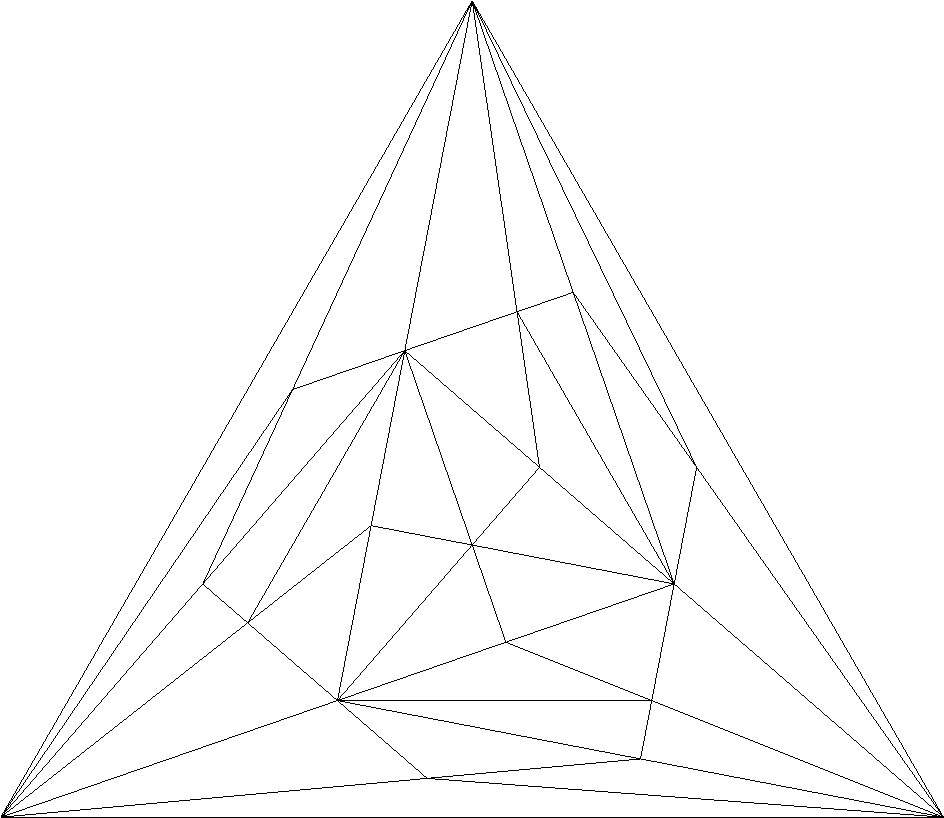
\includegraphics[scale=.2]{renderI}\hspace{.5cm}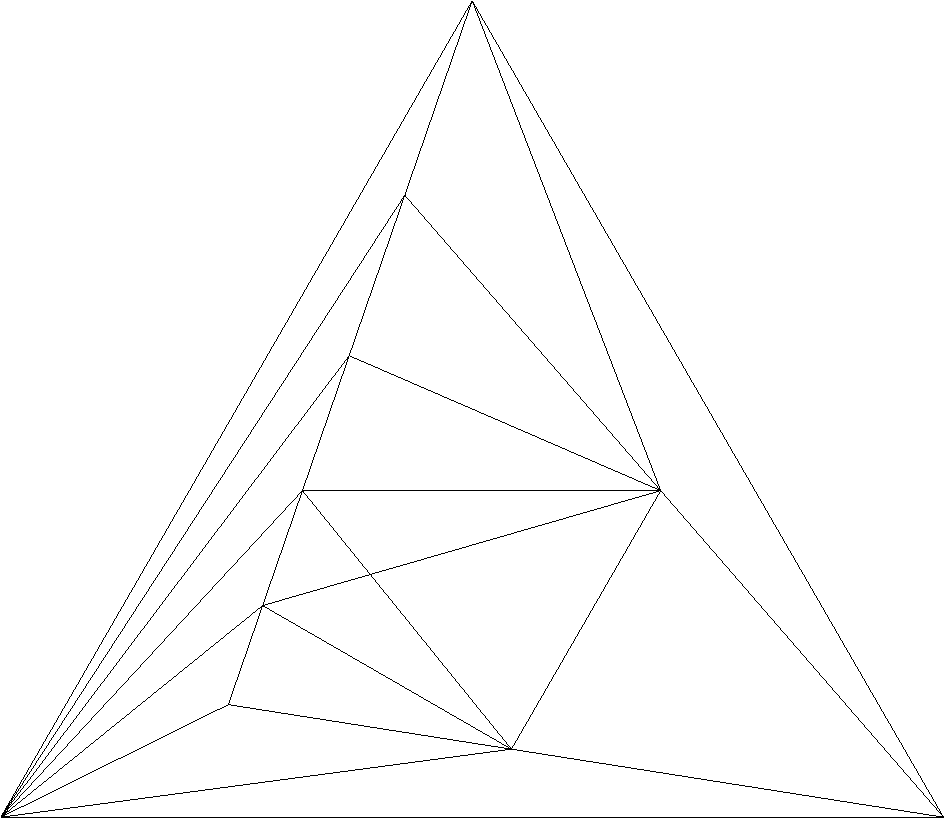
\includegraphics[scale=.2]{renderJ}\caption{Renderings of $\Sigma(I)$ (left) and $\Sigma(J)$ (right), each intersected with the 2-simplex.}\label{fig1}\end{centering}
\end{figure}
\end{example}
\subsection{Tropical Varieties and Tropicalization}
\label{deftrop}
In general, tropical algebraic geometry is the study of the \emph{tropical semiring} $(\RR,\oplus,\odot)$, where $a\oplus b:=\min\{a,b\}$ and $a\odot b:=a+b$. We often may discuss tropical geometry without explicit reference to $\oplus$ and $\otimes$ via a process called \emph{tropicalization}, which gives a correspondence between a variety and its \say{tropicalized} counterpart. In this section, we largely follow \cite[\S3]{MaSt15}. 

 We let $f(x)=\sum_{\vec{u}\in \NN^{n}}c_{\vec{u}}x^{\vec{u}}\in \KK[x]$ We may then define the \emph{tropicalization} of $f$ as a function $\mathrm{trop}(f):\RR^{n}\to \RR$ by \begin{equation} \mathrm{trop}(f)(\vec{w})=\min_{u\in \NN^{n+1}} \{\mathrm{val}(c_{\vec{u}})+\vec{w}\cdot\vec{u}\;:\;\vec{u}\in \NN^{n}\}
\end{equation}
Intuitively, what tropicalization \say{does} is \say{translate} the coefficients of $f$ to $\RR$ with the valuation map and evaluate $f$ at $\vec{u}$ with tropical operations substituted in for their classical counterparts. Now, the graph of $\trop(f)$ over $\RR^{n}$ is a piecewise linear \say{tent} with \say{(tent) poles}\footnote{Yes, this is confusing terminology; we use it only colloquially and only right now with the caution that we are \emph{not} referring to poles in the sense of analysis.} where $\trop(f)$ fails to be differentiable, that is to say where the minimum in its definition is achieved at least twice. We define $\Tcal(f)$, the \emph{tropical hypersurface associated to $f$} as precisely those points in $\RR^{n}$ at which $\trop(f)$ fails to be differentiable. When $n=2$, $\Tcal(f)$ is an embedding of a connected graph into $\RR^2$, pointing towards the central motif of tropical algebraic geometry: transforming data related to smooth varieties into combinatorial data.

Pushing this idea further, we may define the tropical variety of an ideal $I$ as $$\Vcal(I):=\bigcap_{f\in I}\Tcal(f).$$
This is the definition which shall serve as our intuitive understanding of tropical varieties. From the fundamental theorem of tropical algebraic geometry, we may also take the definition of $\Vcal(I)$ to be (i) the set of all vectors $\vec{w}\in \RR^n$ with $\ins_\vec{w}(I)\neq \idl{1}$, or (ii) letting $X=V(I)\subset (\KK^*)^n$, the closure of the image of the coordinate-wise application of the $\val$ map on $X$. We now a slightly modified theorem which shall shed light on the structure of the tropical Grassmannian. \begin{theorem}[Structure Theorem for Tropical Varieties]\label{struc}
If $V(I)$ is an irreducible $d$-dimensional variety in $(\KK^*)^n$, then $\Vcal(I)$ is the support of a pure dimension-$d$ rational polyhedral complex. In particular, if $I$ has a generating set $F$ with \emph{constant coefficients} in the sense that $\val{a_\vec{u}}=0$ for any coefficient $a_\vec{u}$ of $f\in F$, $\Vcal(I)$ is a pure dimension-$d$ fan in $\RR^{n}$.
\end{theorem}
In particular, $\Vcal(I)$ is a subcomplex of the Gr\"obner complex $\Sigma(I_\proj)$.
We use the third definition of $\Vcal(I)$ to define the totally positive part of a tropical variety as $\Vcal^+(I)=\acl{\val(V(I)\cap (\KK^+)}$, that is the closure of the image of the restriction of the valuation map to the totally positive part of the classical variety $V(I)$. Speyer and Williams \cite{WiSp05} prove that a point $\vec{w}\in \Vcal(I)$ lies in $\Vcal^+(I)$ if and only if $\ins_\vec{w}(I)$ contains no nonzero elements of $\RR^+[x_1,\hdots,x_n]$.

\section{Total Positivity, $\trop \left(\gr^+_{k,n}\right)$ and the ``Speyer--Williams Fan" $F_{k,n}$}
\subsection{The Tropical Grassmannian}\label{tropr}
In this section, we work largely from Speyer and Sturmfels' paper \cite{SpSt04} of the same title as well as \cite[\S4.3]{MaSt15}. Theorem \ref{struc} implies that $\trop \left(\gr_{k,n}(\Rcal)\right)$ is a pure $k(n-k)$-dimensional polyhedral fan in $\Rcal^{N}$. Its cones have a common intersection which may be parametrized by the map $\trop \phi: \RR^n\to \trop(\gr_{k,n}(\Rcal))$ which takes $(i_1,\hdots i_n)$ to the ${n\choose k}$-vector which for $K={j_1,j_2,\hdots,j_k}\in {[n]\choose k}$ has $K$-coordinate $i_{j_1}+i_{j_2}+\hdots +i_{j_k}$. $\trop\phi$ is in fact an injection, and thus its image is a pure $n$-dimensional cone. We may also consider $\phi:(\KK^+)^n\to \gr_{k,n}(\KK)$, the de-tropicalization of $\trop \phi$, which maps $(i_1,\hdots i_n)$ to the ${n\choose k}$-vector with $K$-coordinate $i_{j_1}i_{j_2}\hdots i_{j_k}$. Consider the $(\KK^*)^n$-action on $\gr_{k,n}(\KK)$, in which an element $(\lambda_1,\hdots,\lambda_n)\in(\KK^*)^n$ acts on a $k\times n$ matrix $A$ representing a point $P\in \gr_{k,n}(\KK)$ by multiplying each column $i$ by $\lambda_i$. This takes the \plu coordinate $p_K$ to $\left(\prod_{i\in K}\lambda_i\right)p_k$. Then, $\gr_{k,n}(\KK)/\phi((\KK^*)^n)$ is as a set the orbits of the $(\KK^*)^n$-action we have just described. In the next section, we shall discuss a bijective parametrization of this quotient.  
\subsection{Parametrizing the classical Grassmannian and its quotients}
Postnikov has given an explicitly combinatorial parametrization of the Grassmannian \cite{postnikov2006total}, which is generalized by Speyer--Williams \cite{WiSp05} in their study of tropical total positivity, which we follow along with from here. In this  Postnikov's method associates the directed graph $\web_{k,n}$ with $\gr^+_{k,n}$, where $\web_{k,n}$ is the directed graph obtained from a $k\times (n-k)$ grid with rows indexed $1,\hdots,k$ and columns indexed $(k+1),\hdots n$ by adding left- and down-facing arrows to each vertex (as well as sources labeled by $[k]$ along the right side of the grid and sinks labeled by $[n]\setminus [k]$ along the bottom with all labellings increasing clockwise). Each edge is given weighting $x_e$, and a path (compatible with the orientation of the graph) $e_1e_2\hdots e_m$ is associated to the monomial $\prad_p(x)=\prod_{i=1}^mx_{e_{i}}$. For a set of paths $S$, we let $\prad_S(x)=\prod_{p\in S}\prad_p(x)$. We then let $A_{n,k}$ be the $k\times n$ matrix with entries $a_{ij}(x)=(-1)^{i+1}\sum\prad_p(x)$ summing over all paths from the source at vertex $i$ to the sink at vertex $j$. We let $K\in {[n]\choose k}$ and let $\mathrm{Path(K)}$ be the set of tuples of pairwise vertex-disjoint paths with sinks in $K$ and sources in its complement. An application of the familiar  Gessel-Viennot trick for determinental calculations (for an exposition thereof see e.g. \cite[\S2.7]{stan}) yields the following result:\begin{proposition}
	$P_K(x):=p_K(A_{k,n}(x))=\sum_{S\in \mathrm{Path}(k)} \prad_S(x)$. 
\end{proposition}  
Then, substituting elements of $\RR^+$ for the $2k(n-k)$ weight variables $x_e$ gives the Pl\"ucker coordinates of element of $\gr_{3,6}^+(\RR)$.
 This gives a map $\Phi_0:(\RR^+)^{2k(n-k)}\to \gr_{3,6}^+(\RR)$, which, as it turns out, is surjective but due to obvious dimension concerns, is not injective. Speyer and Williams refine this map by replacing the weighting scheme as follows:
  rather than weighting by \emph{edges}, we weight by \emph{regions}, which are defined as follows: inner regions are the maximal connected components of the complement of an embedding of $\web_{k,n}$ into $\RR^2$, while outer regions are those which would satisfy the definition of inner region if we added edges between each source/sink $i$ and $i+1$, but are not inner regions.
  These regions are weighted by monomials $z_r$ in $\{x_e\}$ and $\{x_e^{-1}\}$, with each counterclockwise-oriented edge $e$ bordering region $r$ contributing $x_e$ and each counterclockwise edge $f$ contributing $x_f^{-1}$. Then, one may check that indeed the path monomials $\prad_p(x)$ may be viewed as monomials in the $z_r$, giving a map $\Phi_1:(\RR^+)^{k(n-k)}\to \gr_{k,n}^+(\RR)$.
  Speyer and Williams explicitly construct an inverse map $\Psi$ to $\Phi_1$, showing bijectivity. 
  A key feature of the map $\Psi$ is that each coordinate map (indexing $\RR^{k(n-k)})$ by $[k]\times [j]$) $\Psi_{i,j}$ is the ratio of two monomials in the \plu coordinates $p_{K}$. Thus, the composition $\Psi\Phi_1:(\RR^+)^{k(n-k)}\to(\RR^+)^{k(n-k)}$ expresses each region variable $x_r$ as a ratio of monomials in $P_K(x)$. In particular, the multiset formed from the indices of the numerator of $x_R$ and that formed from the denominator coincide if and only if $R$ is an inner region. Thus, the composition of $\Psi$ with the map $\phi$ of section \ref{tropr} fixes the $x_r$ corresponding to the\ddf{orbits?} inner regions, while acting transitively on the $x_r$ corresponding to the outer regions. This observation gives a bijective map $\Phi_2:(\RR^+)^{(n-k-1)(k-1)}\to\gr^+_{k,n}(\RR) /\phi(\RR^+)^n$ by lifting $c\in (\RR^+)^{(n-k-1)(k-1)}$ to a point $\tilde{c}\in (\RR^+)^{k(n-k)}$ agreeing on the coordinates corresponding to the inner regions, applying $\Phi_1$, then going down to the corresponding point in the quotient. Speyer and Williams also prove that the results above still apply when $\RR^+$ is replaced with $\Rcal^+$, establishing a bijection between $(\Rcal^+)^{(k-1)(n-k-1)}$ and $\gr_{k,n}^+(\Rcal)/\phi(\Rcal^+)^n$. Then, the tropicalization of $\Phi_2$ gives a surjective map $\trop\Phi_2:\RR^{(k-1)(n-k-1)}\to \trop\gr_{k,n}^+/\trop\phi(\RR^+)^n$.
  
  \subsection{The Speyer--Williams Fan} We have now built up the machinery to define the central object of Speyer and Williams' study:
  \begin{definition}
  	The Speyer--Williams fan $F_{k,n}$ is the complete fan in $\RR^{(k-1)(n-k-1)}$ which has as its maximal cones the domains of linearity for $\trop\phi_2$. 
  \end{definition}
Speyer and Williams then show the following results:
\begin{theorem}[\cite{WiSp05}, \S 5-7]~
\begin{enumerate}
	\item The fan $F_{2,n}$ is combinatorially equivalent to the \emph{Stanley--Pitman} fan $F_{n-3}$, which has structure determined by the set of plane binary trees with $n-1$ leaves. The face poset of $F_{2,n}$ adjoined with a maximal element $\hat{1}$ corresponds with that of the type $A_{n-3}$ associahedron.
	\item The fan $F_{3,6}$ has $f$-vector $(16, 66, 98, 48)$, which very nearly coincides with the $f$-vector $(16,66,100,50)$ of the fan normal to the type-$D_4$ generalized associahedron associated to the cluster algebra of type $D_4$. The discrepancy in the latter two coordinates can be explained by noting that two of the cones in $F_{3,6}$ are \say{cones over a bipyramid} which, when subdivided, yield a refined polyhedral complex with $f$-vector coinciding with that of the fan normal to the type-$D_4$ generalized associahedron.
	\item The fan $F_{3,7}$ has $f$-vector $(42, 392, 1463, 2583, 2163, 693)$. There exists a refinement of $F_{3,7}$ which establishes a polyhedral complex with $f$-vector coinciding with that of the fan normal to the type-$E_6$ generalized associahedron, $(42, 399, 1547, 2856, 2499, 833)$.
\end{enumerate}
\end{theorem}
 
In later work, Brodsky, Ceballos, and Labb\'e \cite{BCL16} make the connection between $F_{3,6}$ and type-$D_4$ cluster algebras more precise by giving an explicit bijection between combinatorial types of tropical planes in tropical projective space $\TT\PP^5$, which are realized by $\trop\gr_{3,6}$, and clusters in the cluster algebra of type $D_4$ 
  
\begin{example}
It is (perhaps surprisingly) quite feasible to compute the type-(2,6) Speyer--Williams fan mostly by hand.  Using the inner region construction of $\Phi_2$, no algorithm more sophisticated than heuristic reasoning is required to enumerate every relevant set of lattice paths on the $2\times 4$ rectangular grid network for each $K:=\{i,j\}\in {[6]\choose 2}$. Labeling our three inner-region variables (corresponding right-to-left to the three regions on the left side of the first row) $R_1,R_2,R_3$, we explicitly computed the coordinate functions $P_K(\vec{R})$ of $\Phi_2(\vec{R}):(\RR^+)^3\to \gr^+_{2,6}(\RR) /\phi(\RR^+)^6$. We found that for most $K\in {[6]\choose 2}$, $P_K$ was a monomial and hence when tropicalized, linear everywhere\textemdash this was the case for all $K$ except for $\{2,4\},\{2,5\},\{2,6\},\{3,5\},\{3,6\},\{4,6\}$. In table \ref{eqntable}, we give each $P_K$ for these $K$, which can be read as the coordinate functions for $\Phi_2$ if multiplication and addition are interpreted in the standard sense, or coordinate functions for $\trop \Phi_2$ if they are interpreted as tropical operations. We give as well the domains of linearity for their tropicalization in terms of inequalities, with one cone listed per line of the table. 

After computing each fan $F'_K$ with maximal cones as in the third column of table \ref{eqntable}, we used \verb|polymake| \cite{polymake} to compute their common refinement, yielding the Speyer--Williams fan $F_{2,6}$. We computed that $F_{2,6}$ has 14 maximal cones, which may be written as nonnegative-linear combinations of nine rays. In order to verify our results, we computed its $f$-vector and checked it against the $f$-vector of the type $A_{3}$ associahedron \cite{Pmatrix}. As desired, we found it to have $f$-vector $(1,1,9,21,14)$, which coincides with that of the type-$A_3$ associahedron when the latter four coordinates are reversed in order. As a gallery of the data we generated, we present the rays generating $F_{2,6}$ in table \ref{rays}, the Hasse diagram of its face poset in figure \ref{hasse}, and a visualization of $F_{2,6}$ intersected with the unit ball in figure \ref{visual}\label{mex}.\end{example}\newpage\subsection{Tables and Figures for Example \ref{mex}}\begin{table}[h!]\begin{centering} \begin{tabular}{l|l|l}
			&$P_k(\vec{R})$&$\trop P_k$ domains of linearity\\\hline $P_{24}$& $1+R_1$& $R_1\geq 0$\\&&$R_1\leq 0$\\
			\hline $P_{25}$& $1+R_1(1+R_2)$&$R_1\geq 0$, $R_1+R_2\geq 0$\\&&$R_1\leq 0$, $R_2\geq 0$\\&&$R_1+R_2\leq 0$, $R_2\leq 0$\\
			\hline $P_{26}$& $1+R_1(1+R_2(1+R_3))$&$R_1\geq 0$, $R_1+R_2\geq 0$, $R_1+R_2+R_3\geq 0$\\
			&&$R_1\leq 0$, $R_2\geq 0$, $R_2+R_3\geq 0$\\
			&&$R_1+R_2\leq 0$, $R_2\leq 0$, $R_3\geq 0$\\
			&&$R_1+R_2+R_3\leq 0$, $R_2+R_3\leq 0$, $R_3\leq 0$\\
			\hline $P_{35}$&$R_1(1+R_2)$&$R_2\geq 0$\\&&$R_2\leq 0$\\
			\hline $P_{36}$&$R_1(1+R_2(1+R_3))$&$R_2+R_3\geq 0$, $R_2\geq 0$\\&&$R_2\leq 0$, $R_3\geq 0$\\&&$R_3\leq 0 $, $R_2+R_3\leq 0$\\
			\hline $P_{4,6}$& $R_1R_2(1+R_3)$&$R_3\geq 0$\\
			&&$R_3\leq 0$
			
		\end{tabular}
		\caption{\label{eqntable}$P_K(\vec{R})$ for each non-monomial $P_K$, and the domains of linearity for $\trop P_K$.}\end{centering}
\end{table}
\begin{table}[h!]\begin{centering}
	\begin{tabular}{c|c}
		Label & Ray\\
		\hline\hline
	0&	$(1, 0, 0)$\\
	1&$(0, 1, 0)$\\
2&	$(	0, 0 ,1)$\\
3&		$(-1, 0, 0)$\\
4&		$(0, 1, -1)$\\
5&		$(1, 0 ,-1)$\\
6&$(		0, 0 ,-1)$\\
7&$		(1 ,-1, 0)$\\
8&$		(0 ,-1, 0)$\\
		
	\end{tabular}\caption{The rays used to describe the cones of $F_{2,6}$\label{rays}}\end{centering}
\end{table}
\begin{figure}[h!]\begin{centering}
	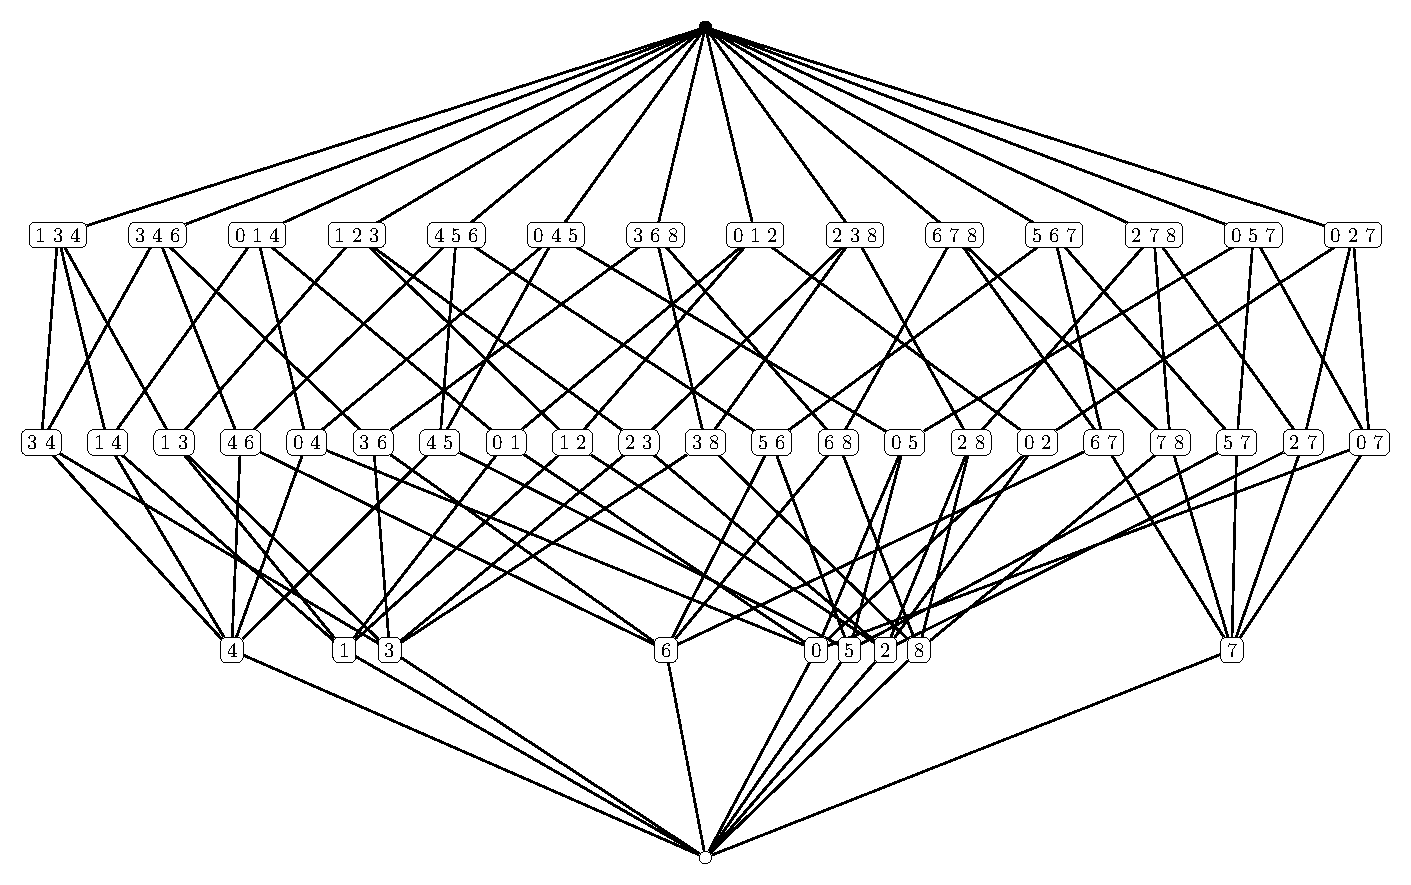
\includegraphics[scale=.55]{f5h}\caption{\label{hasse} Hasse diagram of the face poset of $F_{2,6}$. Labeling of nodes corresponds to the rays which generate the cone corresponding to that node (see table \ref{rays}).}\end{centering}
\end{figure}
\begin{figure}[h!]\begin{centering}
		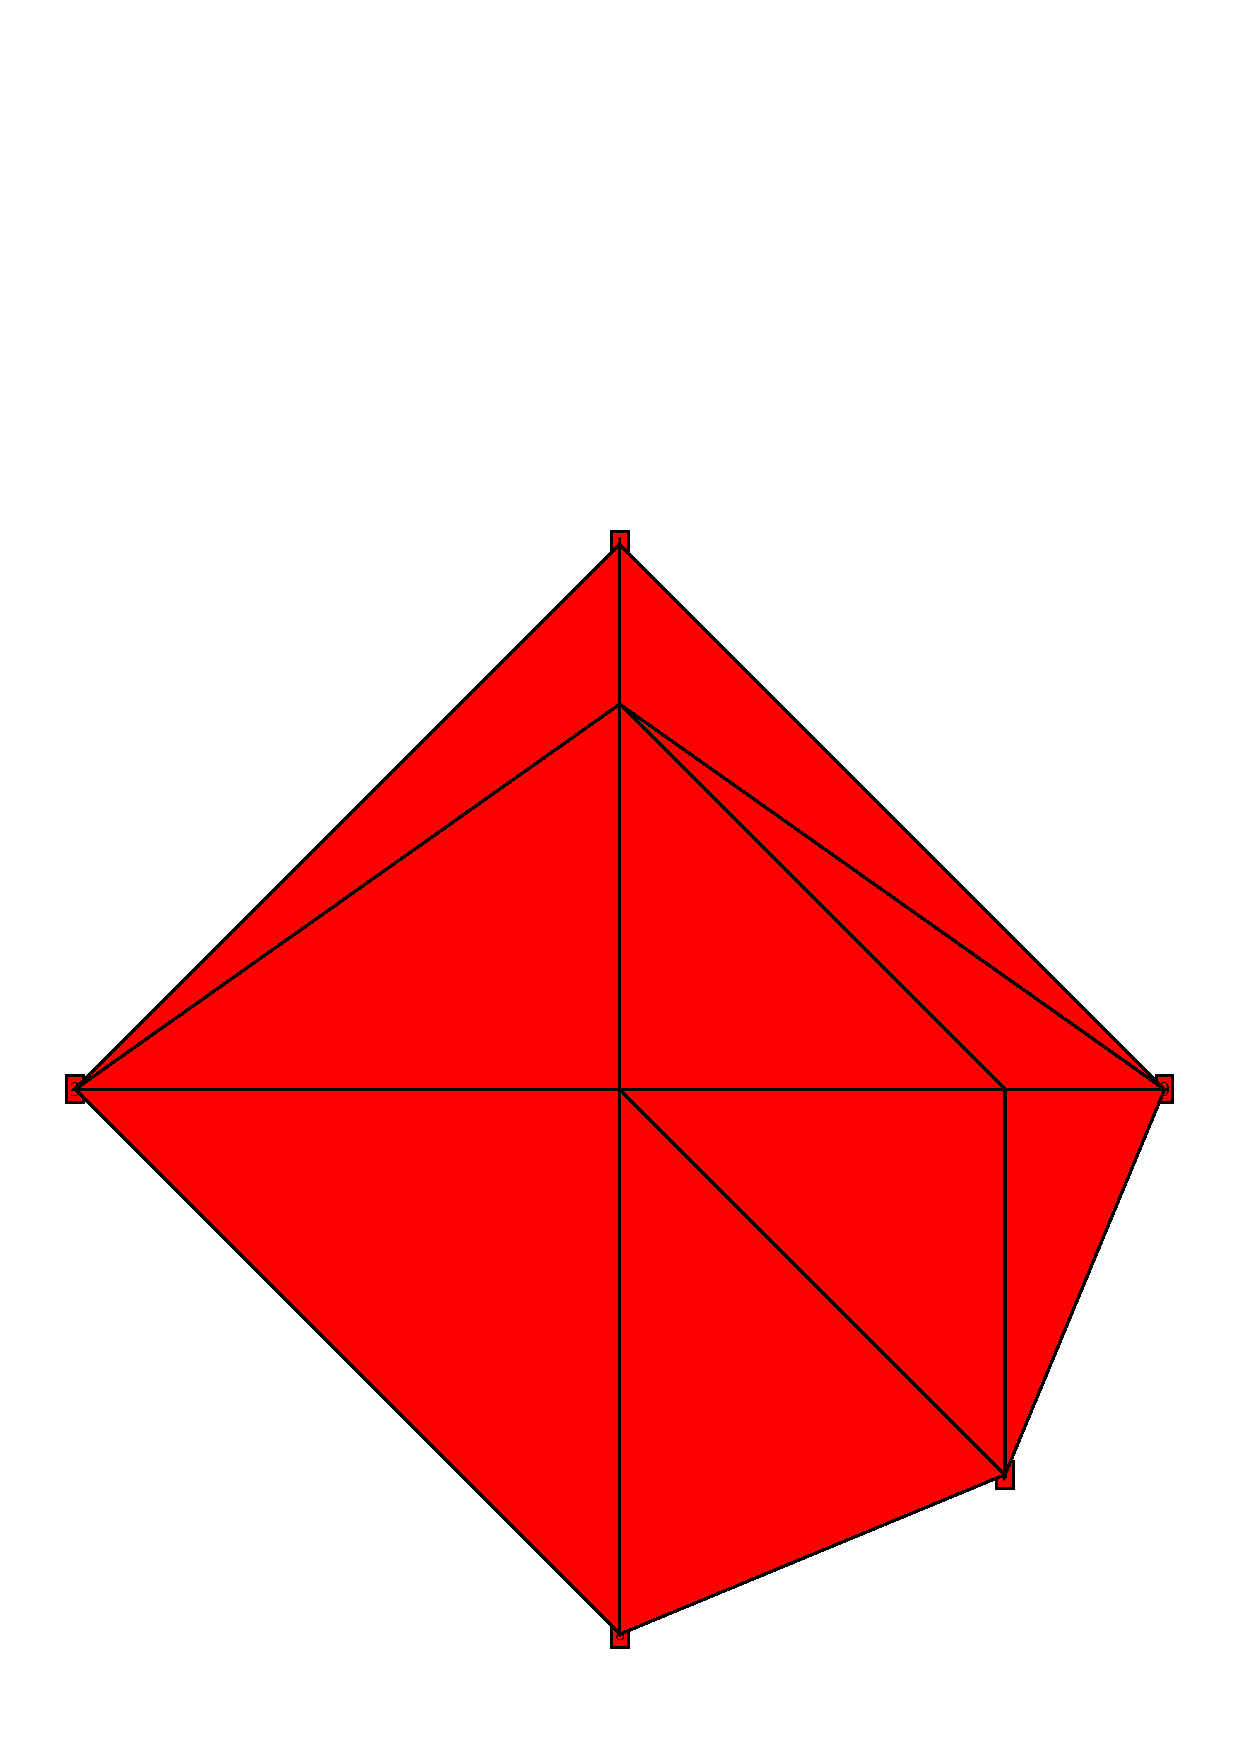
\includegraphics[scale=.3]{f5v}\caption{\label{visual}Rendering of $F_{2,6}$, intersected with the unit ball.}\end{centering}
\end{figure}
\newpage
%We have now built up the machinery we need to define the Speyer--Williams fan $F_{k,n}$. 
%\section{Computing the $f$-vector of $F_{3,6}$}
\nocite{*}
\printbibliography
\end{document}
